\documentclass[12pt, hyperref={bookmarks=false}, show notes]{beamer}
% Switch to this for handouts
%\documentclass[12pt,handout]{beamer}

% Text
	\usepackage[T1]{fontenc}
  %\usepackage{emerald}
	\usepackage[utf8]{inputenc}
	\usepackage[english]{babel}
	% \usepackage[bitstream-charter]{mathdesign} % Serif font (Charter BT).
	\usepackage[scaled=0.84]{DejaVuSansMono} % Monospaced font.
	\def\sfdefault{SourceSansPro-TLF} % Sans serif font.
	\usepackage{textcomp}

% Maths
  \usepackage{amsmath}
  \usepackage{mathtools}
  \usepackage{siunitx}

% Graphics
  \usepackage{graphicx}
  \usepackage[caption=false]{subfig}
  \usepackage{tikz}
  \usepackage{bchart}
  \usepackage{pgfplots}
  \pgfplotsset{compat=1.10}
	% ADD TIKZ LIBRARIES
  \usetikzlibrary{calc}
  \usetikzlibrary{arrows.meta}
  %\usepackage{tikz-qtree}
  \usetikzlibrary{decorations.pathmorphing}
  \usetikzlibrary{matrix,shapes,positioning,fit}
  \usepgfplotslibrary{external}
  \tikzexternalize[prefix=gfx/tikz/]
  \tikzexternaldisable % Disable by default

  \tikzstyle{bigblock} = [thick, rectangle, draw, fill=clnode, text width=4.5em, text centered, minimum height=4em]
  \tikzstyle{smallblock} = [thick, rectangle, draw, fill=clnode, text width=4.5em, text centered, minimum height=3em]
  \tikzstyle{database} = [thick, cylinder, draw, shape border rotate=90, aspect=0.15, fill=clnode, text width=3em, text centered, minimum height=4em]
  \tikzstyle{line} = [draw, -stealth, thick]
  %\tikzstyle{model} = [draw, ellipse,fill=red!20, minimum height=2em]
  \tikzstyle{container} = [rectangle, draw, inner sep=0.6 cm, dashed, fill=clshade]
  \tikzstyle{node} = [thick, circle, draw, fill=clnode, text width=1.5em, text centered, minimum height=1.5em]
  
  \usepackage{pgfgantt}
  \usepackage{mdframed}
  \newmdenv [align=center, backgroundcolor=color3!10, linecolor=color3!50, linewidth=1pt]{mtjbox}

	\usepackage{xcolor}
    \definecolor{color1}{cmyk}{100,50,0,0}   % blue
    \definecolor{color2}{cmyk}{0,80,100,0}   % vermillion
    \definecolor{color3}{cmyk}{97,0,75,0}    % blueish green
    \definecolor{color4}{RGB}{204,121,167}    % reddish purple
    \definecolor{color5}{RGB}{230,159,0}   % orange
    \definecolor{clnode}{gray}{0.85}
    \usepackage{colortbl}
% Misc
\usepackage{booktabs}
\usepackage{enumerate}
\usepackage{pdfpages}
\usepackage{pgfpages}
%\usepackage{setspace}
%\usepackage{multimedia}

% Box colors.
\definecolor{clframe}{gray}{0.75}
\definecolor{clshade}{gray}{0.95}
\definecolor{clcodeshade}{gray}{0.93}

% Code colors.
\definecolor{javared}{rgb}{0.6,0,0}            % for strings
\definecolor{javagreen}{rgb}{0.25,0.5,0.35}    % comments
\definecolor{javapurple}{rgb}{0.6,0,0.5}       % keywords
\definecolor{javadocblue}{rgb}{0.25,0.35,0.75} % javadoc

%More colors
\definecolor{colorA}{HTML}{5DA5DA} % blue
\definecolor{colorB}{HTML}{FAA43A} % orange
\definecolor{colorC}{HTML}{60BD68} % green
\definecolor{colorD}{HTML}{F17CB0} % pink
\definecolor{colorE}{HTML}{B2912F} % brown
\definecolor{colorF}{HTML}{B276B2} % purple
\definecolor{colorG}{HTML}{DECF3F} % yellow
\definecolor{colorH}{HTML}{F15854} % red
\definecolor{colorI}{HTML}{4D4D4D} % gray

\colorlet{colorAshade}{colorA!80!black}
\colorlet{colorBshade}{colorB!80!black}
\colorlet{colorCshade}{colorC!80!black}
\colorlet{colorDshade}{colorD!80!black}
\colorlet{colorEshade}{colorE!80!black}
\colorlet{colorFshade}{colorF!80!black}
\colorlet{colorGshade}{colorG!80!black}
\colorlet{colorHshade}{colorH!80!black}
\colorlet{colorIshade}{colorI!80!black}

\usepackage{listings}

\lstdefinestyle{javastyle}{%
  language=Java,
  keywordstyle=\color{javapurple}\bfseries,
  stringstyle=\color{javared},
  commentstyle=\color{javagreen},
  morecomment=[s][\color{javadocblue}]{/**}{*/}
}

\lstnewenvironment{javacode}[1][]{%
  \lstset{style=javastyle, #1}
}{}

\lstset{
  columns=flexible,
  escapechar=",
  escapeinside={(*@}{@*)},
  basicstyle=\ttfamily\footnotesize,
  frame=single, backgroundcolor=\color{clshade}, rulecolor=\color{clframe},
  framerule=\fboxrule, xleftmargin=3.4pt, xrightmargin=3.4pt, belowskip=\smallskipamount,
  captionpos=b,
  numbers=left,
  numberstyle=\scriptsize,
  numbersep=7pt,
  tabsize=2,
  keepspaces=true,
  showspaces=false,
  showstringspaces=false,
  breaklines=true,
  breakatwhitespace=true,
  postbreak=\raisebox{0ex}[0ex][0ex]{\ensuremath{\color{red}\hookrightarrow\space}}
}



\setbeamertemplate{navigation symbols}{}
%\setbeamertemplate{bibliography item}[text]

%\usepackage{caption}
\usetheme{/amsterdam}
\date{June 15, 2015}

%Uncomment for handouts: (remember to uncomment in line 1+2, too)
%\usepackage{beamertheme/handoutWithNotes}
%\pgfpagesuselayout{4 on 1 with notes}[a4paper,border shrink=5mm]

% Comment for handouts or slides without notes:
\setbeameroption{show notes on second screen=right}
\setbeamertemplate{note page}{%
  \insertnote%
}

% Table of content dybde (0-index)
%\setcounter{tocdepth}{1}

% BibLaTeX
%\usepackage{csquotes}
%\usepackage[
%backend=bibtex,
%citestyle=numeric,
%bibstyle=numeric,
%maxcitenames=3,
%maxbibnames=99,
%url=true]{biblatex}
%\addbibresource{../rapport/references/refs.bib}
%\addbibresource{extrasources.bib}
%\usepackage{../style/biblatex_custom_formatting}

\graphicspath{{gfx/}{../report/graphics/}{../report/graphics/tikz}}

\begin{document}

%\captionsetup[figure]{font=small,singlelinecheck=off,justification=raggedright}

\title[Improving Wikipedia Linking: A Feature Learning Approach]{Improving Wikipedia Linking: A Feature Learning Approach}
% \author[\insertframenumber /\inserttotalframenumber]{sw609f15}
\makeatletter
  \defbeamertemplate*{footline}{myminiframes theme}
  {%
    \begin{beamercolorbox}[colsep=1.5pt]{upper separation line foot}
    \end{beamercolorbox}
    \hbox{%
      \begin{beamercolorbox}[wd=.75\paperwidth,ht=2.5ex,dp=1.125ex,%
        leftskip=.3cm,rightskip=.3cm plus1fil]{title in head/foot}%
        \leavevmode{\usebeamerfont{title in head/foot}\insertshorttitle}%
      \end{beamercolorbox}%
      \begin{beamercolorbox}[wd=.15\paperwidth,ht=2.5ex,dp=1.125ex,%
        leftskip=.3cm,rightskip=.3cm]{title in head/foot}%
        {\usebeamerfont{author in head/foot}\usebeamercolor[fg]{author in head/foot}\insertshortauthor}
      \end{beamercolorbox}%
      \begin{beamercolorbox}[wd=.1\paperwidth,ht=2.5ex,dp=1.125ex,%
        leftskip=.3cm,rightskip=.3cm,center]{title in head/foot}%
        {\usebeamerfont{author in head/foot}\usebeamercolor[fg]{author in head/foot}\insertframenumber/\inserttotalframenumber}%
      \end{beamercolorbox}%
    }%
    \begin{beamercolorbox}[colsep=1.5pt]{lower separation line foot}
    \end{beamercolorbox}
  }
\makeatother

% Adding front slide.
{
\setbeamercolor{background canvas}{bg=}

\includepdf[pages=1]{frontslide.pdf}
}
\note{
    Noter, noter, noter!
}

\begin{frame}
  \frametitle{Contents}
  \tableofcontents
  \note{
  \begin{itemize}
    \item Notes
    \item notes
    \item notes..
  \end{itemize}
}
\end{frame}


\chapter{Introduction}
The World Wide Web is built upon the idea of \emph{creating a space in which anything could be linked to anything} \todo{insert cite: Weaving the Web, chapter 1 by Tim Berners-Lee}. Thus, hyperlinking can be seen as a vital component of the World Wide Web, and even a critical component to its success. Hyperlinking allows websites to be easily navigationable, enabling users to quickly find relevant or in-depth information.

A wide array of research that tries to find links.

\todo{motivation and users}

\section{Problem Statement}
\dummy

\section{Project Goals}
\todo{Success criteria (to be evaluated in the conclusion)}

\section{Compliance with Study Regulation}
\todo{Maybe a description of how the project fits within the study regulation}

\section{Report Organization}
This report describes and documents the design, implementation, evaluation and development method of the system described in this chapter. Immediately following this introduction, \chapterref{chap:analysis} ... \dummy ... \chapterref{chap:devmethodreflection} contains a discussion and reflection of the development process used throughout this project.
\section[System Design Overview]{System Design Overview}
% Første parameter i [] er tekst i header. {} er i indholdsfortegnelsen.

% Slide med emneoverskrift.
\begin{frame}
  \frametitle{}
  \begin{center}
    {\Huge System Design Overview}
  \end{center}
\end{frame}
\note{
  \begin{itemize}
		\item Notes...
  \end{itemize}
}

% Normal slide:
\begin{frame}
    \frametitle{System Design Overview}
    \centering
    \begin{itemize}
      \item System characteristics \& requirements
      \item Design goals
      \item Architecture
    \end{itemize}
\end{frame}

\begin{frame}
    \frametitle{System characteristics \& requirements}
    \centering
    \begin{itemize}
      \item Find article pairs to link
      \item Data processing - backend
      \begin{itemize}
        \item Maintainable
        \item Scalable
      \end{itemize}
      \item Presentation to users - frontend
      \begin{itemize}
        \item Fast response times
      \end{itemize}
    \end{itemize}
\end{frame}
\note{
  \begin{itemize}
		\item We chose machine learning approach - Data processing by nature
    \item Calculation heavy - backend
    \item Maintainable - experimentation + prototyping
    \item Scalable - work with larger datasets
  \end{itemize}
}

\begin{frame}
    \frametitle{Design goals}
    \centering
    \begin{itemize}
      \item Modularity
      \begin{itemize}
        \item Separated components
        \item Data protocol - loose coupling
        \item Individual component development
      \end{itemize}
      \item Scalability
      \begin{itemize}
        \item Distributed components - horizontal scaling
        \item Resolve bottlenecks
        \item Offloading
      \end{itemize}
    \end{itemize}
\end{frame}
\note{
  \begin{itemize}
    \item Adhere to protocol
		\item Individual component development - languages and platforms
    \item Offloading
    \begin{itemize}
      \item Moves work from backend to frontend
      \item More data has to be transfered to the frontend
    \end{itemize}
  \end{itemize}
}

\begin{frame}
    \centering
    \resizebox{\textwidth}{!}{%
      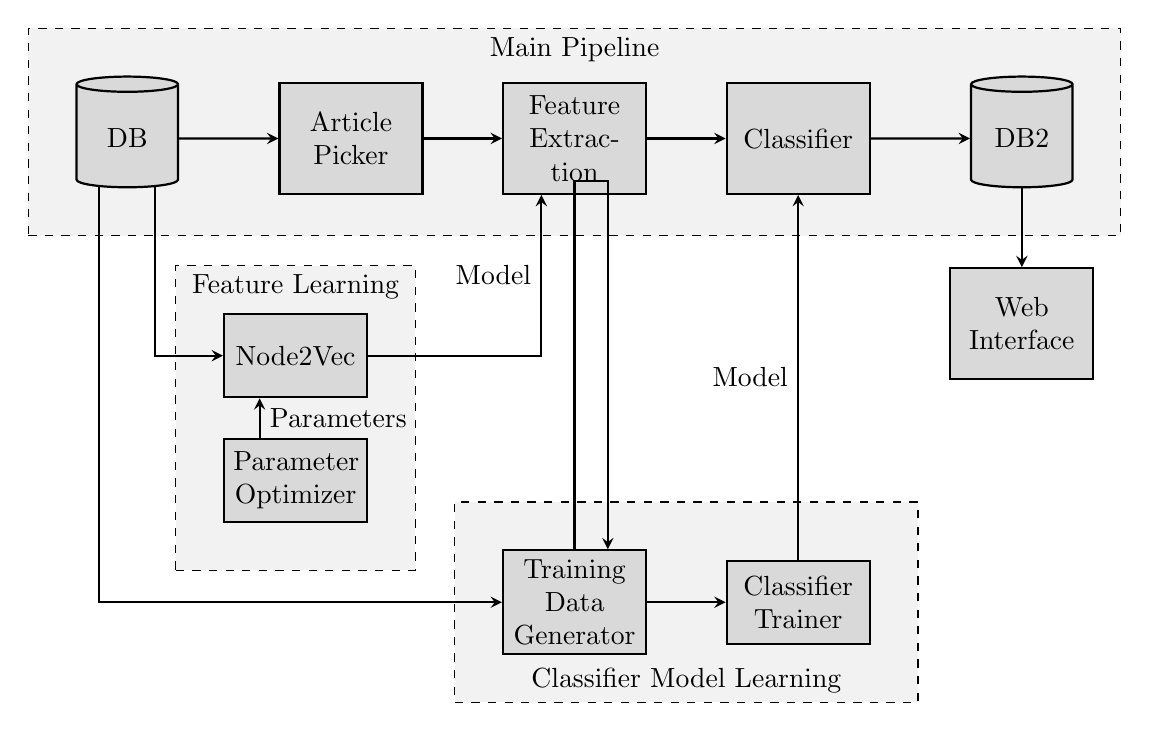
\begin{tikzpicture}[node distance = 2.84cm, auto]
    \node [database, yshift=1em] (db) {DB};
    \node [bigblock, right of=db] (ap) {Article Picker};
    \node [bigblock, right of=ap] (tfl) {Feature Extraction};
    \node [bigblock, right of=tfl] (classifier) {Classifier};
    \node [database, right of=classifier] (db2) {DB2};
    \node [bigblock, below=1cm of db2] (web) {Web Interface};
    
    %\node [above=1cm of ap] (inputarticle) {};
    
    \node [smallblock, below=1.5cm of ap, xshift=-2em] (n2v) {Node2Vec};
    \node [smallblock, below=.5cm of n2v] (paropt) {Parameter Optimizer};
    
    \node [smallblock, below=4.5cm of tfl] (prepper) {Training Data Generator};
    \node [smallblock, right of=prepper] (classifierTrainer) {Classifier Trainer};
    
    \begin{scope}[on background layer]
    \node [container, fit=(n2v)(paropt)] (container1) {};
    \node[below] at (container1.north) {Feature Learning};
    \node [container, fit=(prepper)(classifierTrainer)] (container2) {};
    \node[above] at (container2.south) {Classifier Model Learning};
    
    \node [container, fit=(db)(db2)] (container3) {};
    \node[below] at (container3.north) {Main Pipeline};
    \end{scope}
    
    %\draw [->] (db) -- (n2v);
    
    \path [line] (db) -- (ap);
    %\path [line] (inputarticle) -- (ap);
    \path [line] (ap) -- (tfl);
    \path [line] (tfl) -- (classifier);
    \path [line] (classifier) -- (db2);
    \path [line] (db2) -- (web);
    
    \path [line] (db.300) |- (n2v);
    %\path [line] (db.300) |- (paropt);
    \path [line] (db.240) |- (prepper);
    
    \path [line, swap, transform canvas={xshift=-1.3em}] (paropt) -- node{Parameters} (n2v);
    \path [line] (n2v.east) -| node [near end] {Model} ([xshift=-1.2em]tfl.south);
    
    \path [line] (prepper) -- (classifierTrainer);
    %\path [line] (prepper) -- (tfl);
    %\path [line] ([xshift=1.2em]tfl.south) -- ([xshift=1.2em]prepper.north);
    \draw [line] (prepper.north) |- ([xshift=1.2em, yshift=0.5em]tfl.south) -- ([xshift=1.2em]prepper.north);
    
    \path [line] (classifierTrainer) -- node{Model} (classifier);
    
  \end{tikzpicture}
    }
\end{frame}
\note{
  \begin{itemize}
    \item Pipeline for suggestions
    \item Main pipeline envisioned offline processing
  \end{itemize}
}
\section[Components]{Components Overview}
% Første parameter i [] er tekst i header. {} er i indholdsfortegnelsen.

% Slide med emneoverskrift.
\begin{frame}
  \frametitle{}
  \begin{center}
    {\Huge Components Overview}
  \end{center}
\end{frame}


\begin{frame}
    \centering
    \resizebox{\textwidth}{!}{%
      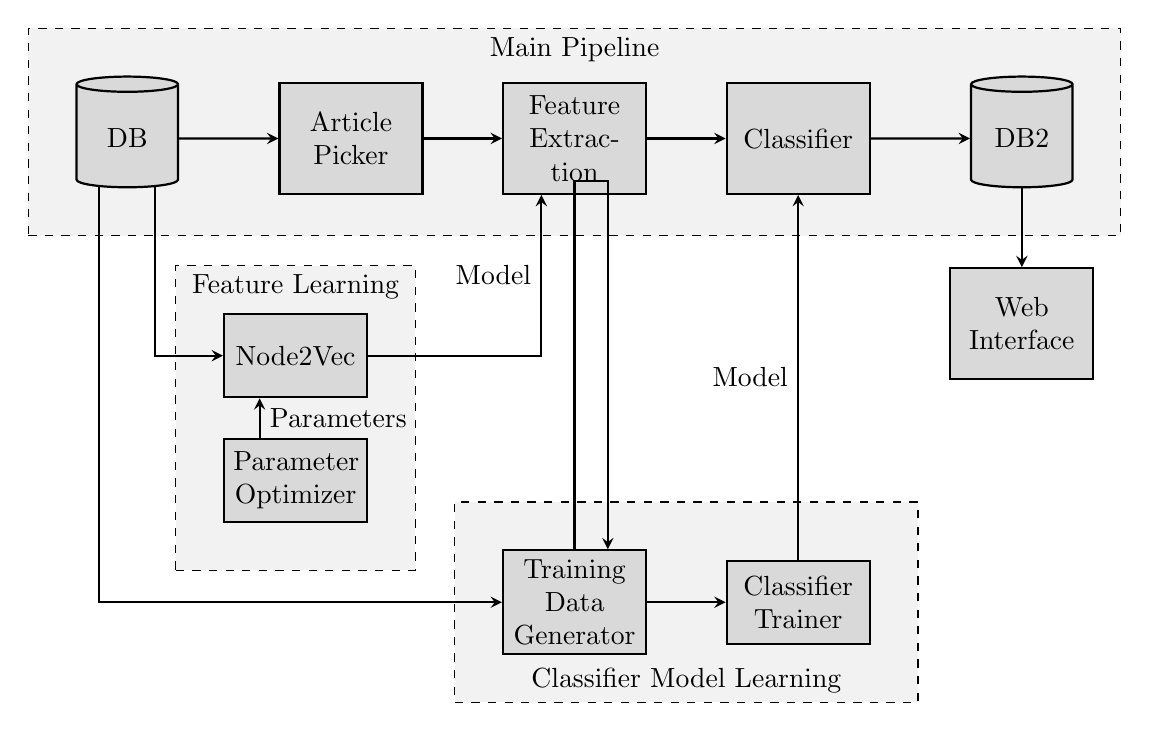
\begin{tikzpicture}[node distance = 2.84cm, auto]
    \node [database, yshift=1em] (db) {DB};
    \node [bigblock, right of=db] (ap) {Article Picker};
    \node [bigblock, right of=ap] (tfl) {Feature Extraction};
    \node [bigblock, right of=tfl] (classifier) {Classifier};
    \node [database, right of=classifier] (db2) {DB2};
    \node [bigblock, below=1cm of db2] (web) {Web Interface};
    
    %\node [above=1cm of ap] (inputarticle) {};
    
    \node [smallblock, below=1.5cm of ap, xshift=-2em] (n2v) {Node2Vec};
    \node [smallblock, below=.5cm of n2v] (paropt) {Parameter Optimizer};
    
    \node [smallblock, below=4.5cm of tfl] (prepper) {Training Data Generator};
    \node [smallblock, right of=prepper] (classifierTrainer) {Classifier Trainer};
    
    \begin{scope}[on background layer]
    \node [container, fit=(n2v)(paropt)] (container1) {};
    \node[below] at (container1.north) {Feature Learning};
    \node [container, fit=(prepper)(classifierTrainer)] (container2) {};
    \node[above] at (container2.south) {Classifier Model Learning};
    
    \node [container, fit=(db)(db2)] (container3) {};
    \node[below] at (container3.north) {Main Pipeline};
    \end{scope}
    
    %\draw [->] (db) -- (n2v);
    
    \path [line] (db) -- (ap);
    %\path [line] (inputarticle) -- (ap);
    \path [line] (ap) -- (tfl);
    \path [line] (tfl) -- (classifier);
    \path [line] (classifier) -- (db2);
    \path [line] (db2) -- (web);
    
    \path [line] (db.300) |- (n2v);
    %\path [line] (db.300) |- (paropt);
    \path [line] (db.240) |- (prepper);
    
    \path [line, swap, transform canvas={xshift=-1.3em}] (paropt) -- node{Parameters} (n2v);
    \path [line] (n2v.east) -| node [near end] {Model} ([xshift=-1.2em]tfl.south);
    
    \path [line] (prepper) -- (classifierTrainer);
    %\path [line] (prepper) -- (tfl);
    %\path [line] ([xshift=1.2em]tfl.south) -- ([xshift=1.2em]prepper.north);
    \draw [line] (prepper.north) |- ([xshift=1.2em, yshift=0.5em]tfl.south) -- ([xshift=1.2em]prepper.north);
    
    \path [line] (classifierTrainer) -- node{Model} (classifier);
    
  \end{tikzpicture}
    }
\end{frame}


% Normal slide:
\begin{frame}
    \frametitle{Database}
    %\framesubtitle{Link Distribution}
    \centering

    \begin{itemize}
      \item DBPedia
      \begin{itemize}
        \item Articles
        \item Links
        \item Redirects
      \end{itemize}
      \item Graph Database
      \begin{itemize}
        \item Queries
        \item Plugins: Random Walks
      \end{itemize}
    \end{itemize}

\end{frame}
\note{
  \begin{itemize}
    \item Graph modeling
    \item Optimized for graphs
  \end{itemize}
}

\begin{frame}
    \frametitle{Database}
    \framesubtitle{Link Distribution}
    \centering

    \begin{itemize}
      \item Total article links: 138,864,625 % (138.422.339)
      \item Links from featured articles: 737,143 (0.53\%)
    \end{itemize}

    
\includegraphics[width=\textwidth]{link-distribution}
\end{frame}
\note{
  \begin{itemize}
    \item Small proportion
    \item Ground truth
  \end{itemize}
}


\begin{frame}
    \frametitle{Feature Learning}
    %\framesubtitle{Data Partitioning}
    \centering

    \begin{itemize}
      \item node2vec
      \item Article features
    \end{itemize}

    
\includegraphics[width=\textwidth]{feature-learning}
\end{frame}
\note{
  \begin{itemize}
    \item Notes here...
  \end{itemize}
}


\begin{frame}
    \frametitle{Feature Extraction}
    %\framesubtitle{Data Partitioning}
    \centering

    \begin{itemize}
      \item Combine article features
      \item non-commutative operation
    \end{itemize}

   
\includegraphics[width=\textwidth]{feature-extractor}
\end{frame}
\note{
  \begin{itemize}
    \item Concatenation
  \end{itemize}
}


\begin{frame}
    \frametitle{Classification}
    %\framesubtitle{Data Partitioning}
    \centering

    \begin{itemize}
      \item 10-fold cross-validation
    \end{itemize}

    
\includegraphics[width=\textwidth]{classifier-training}
\end{frame}
\note{
  \begin{itemize}
    \item Positive/Negative training samples
  \end{itemize}
}


\begin{frame}
    \frametitle{Machine Learning Pipeline}
    \framesubtitle{Components}
    \centering

    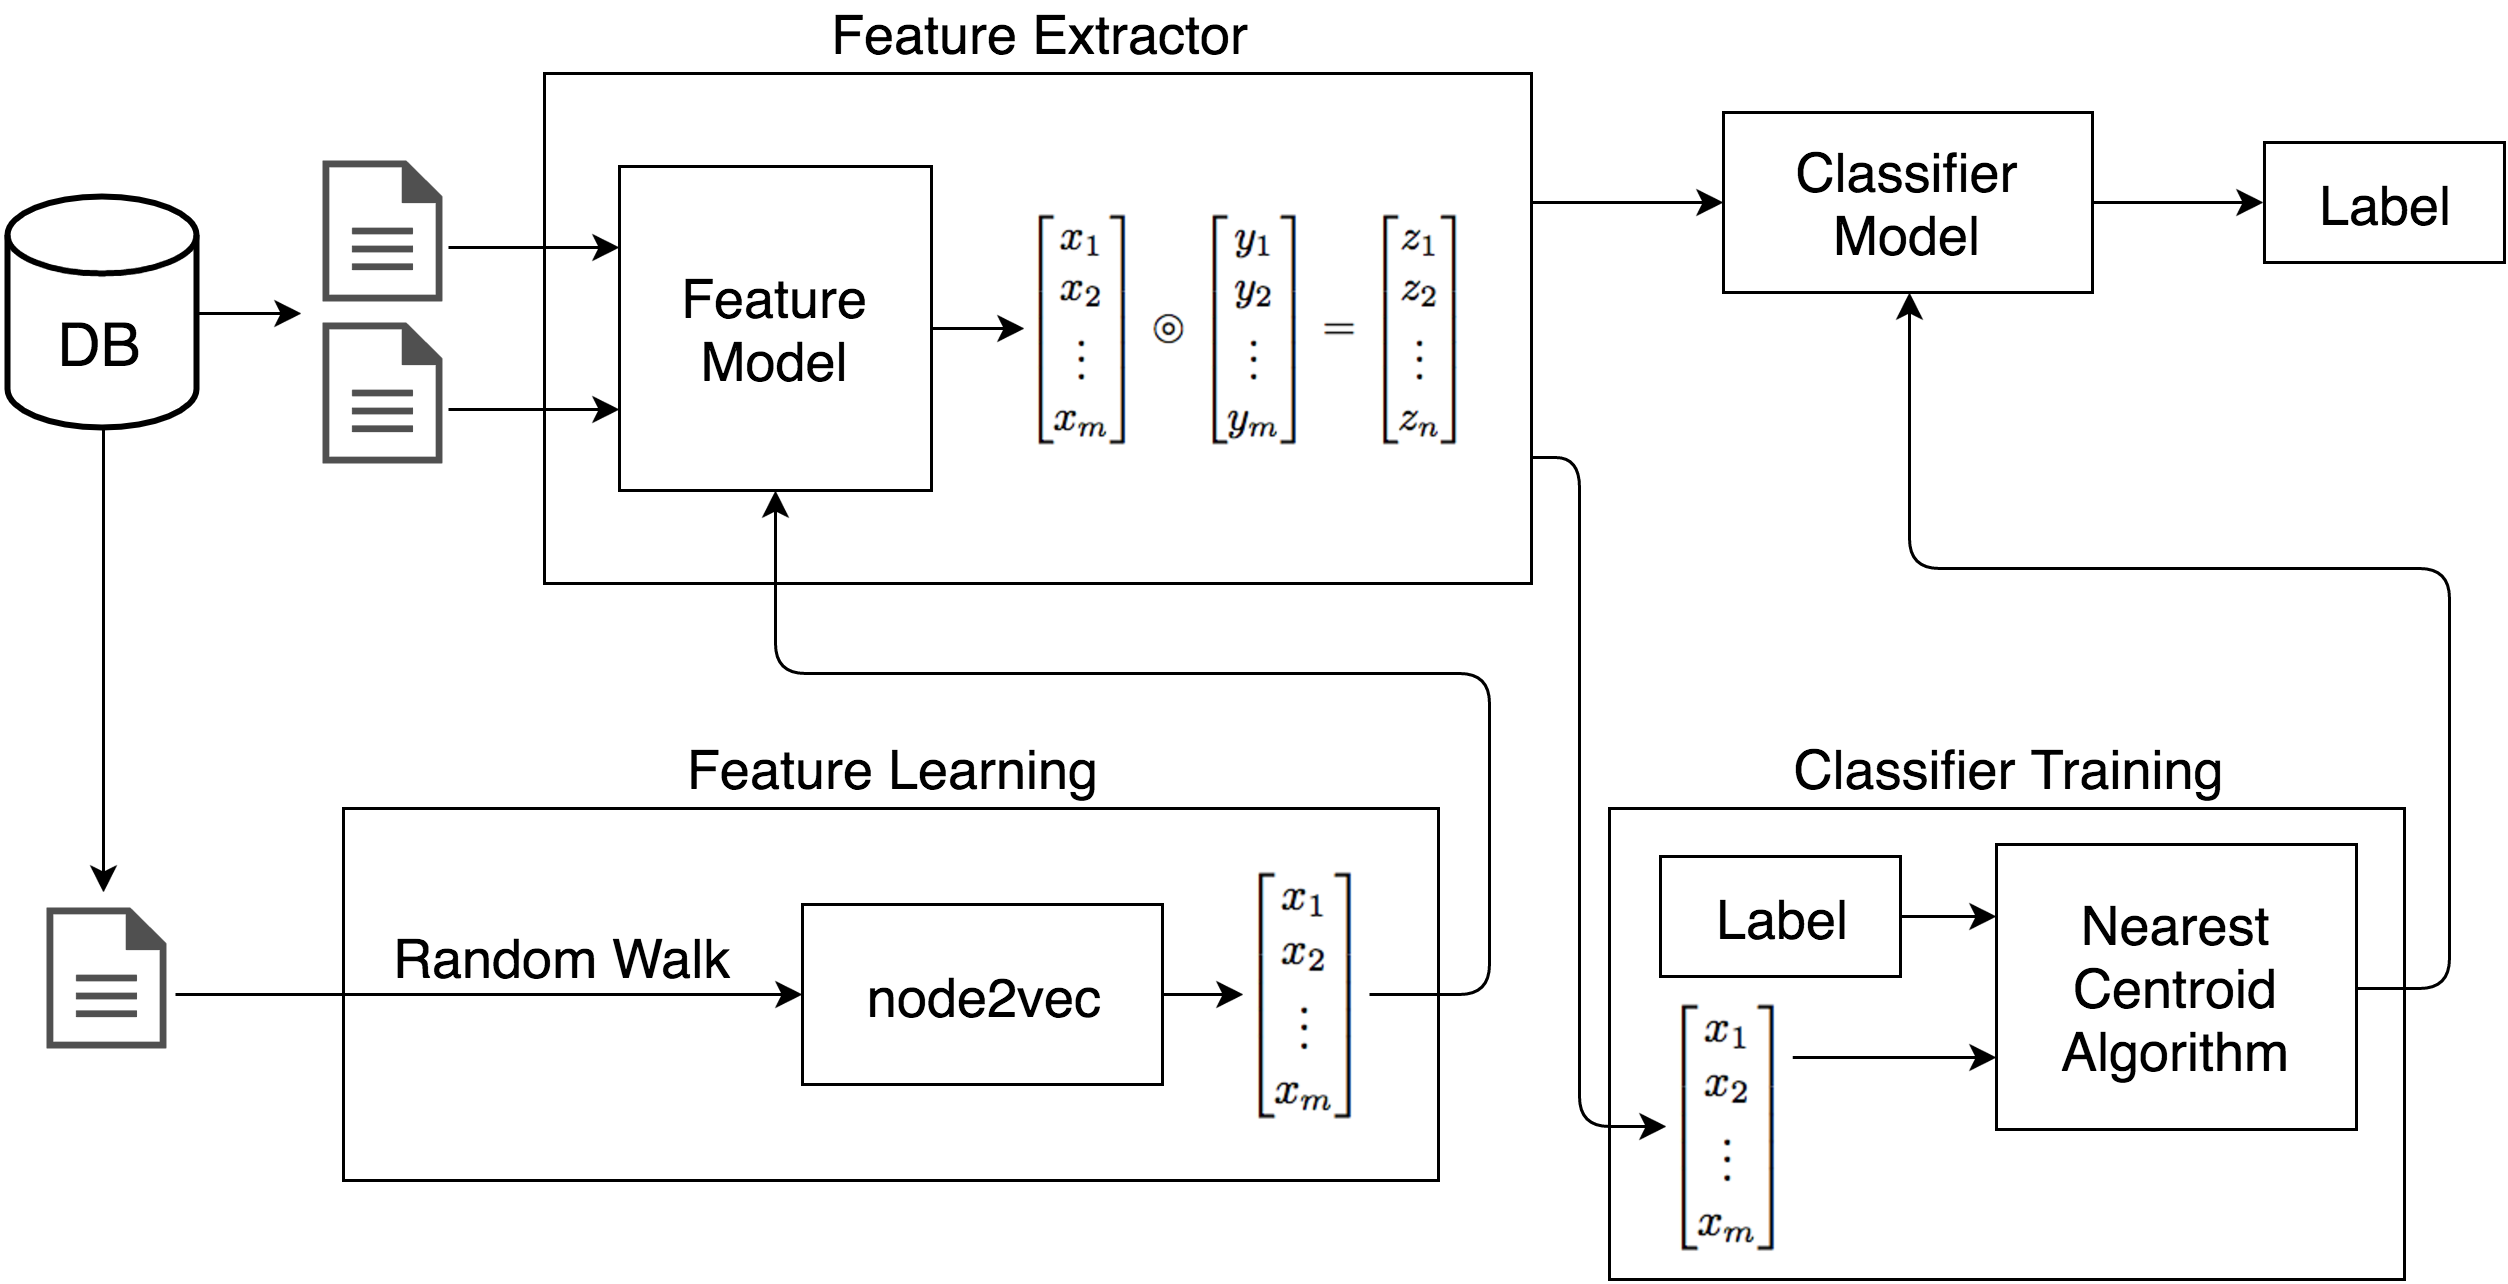
\includegraphics[width=\textwidth]{pipeline}
\end{frame}


\begin{frame}
    \frametitle{Machine Learning Pipeline}
    \framesubtitle{Components}
    \centering

    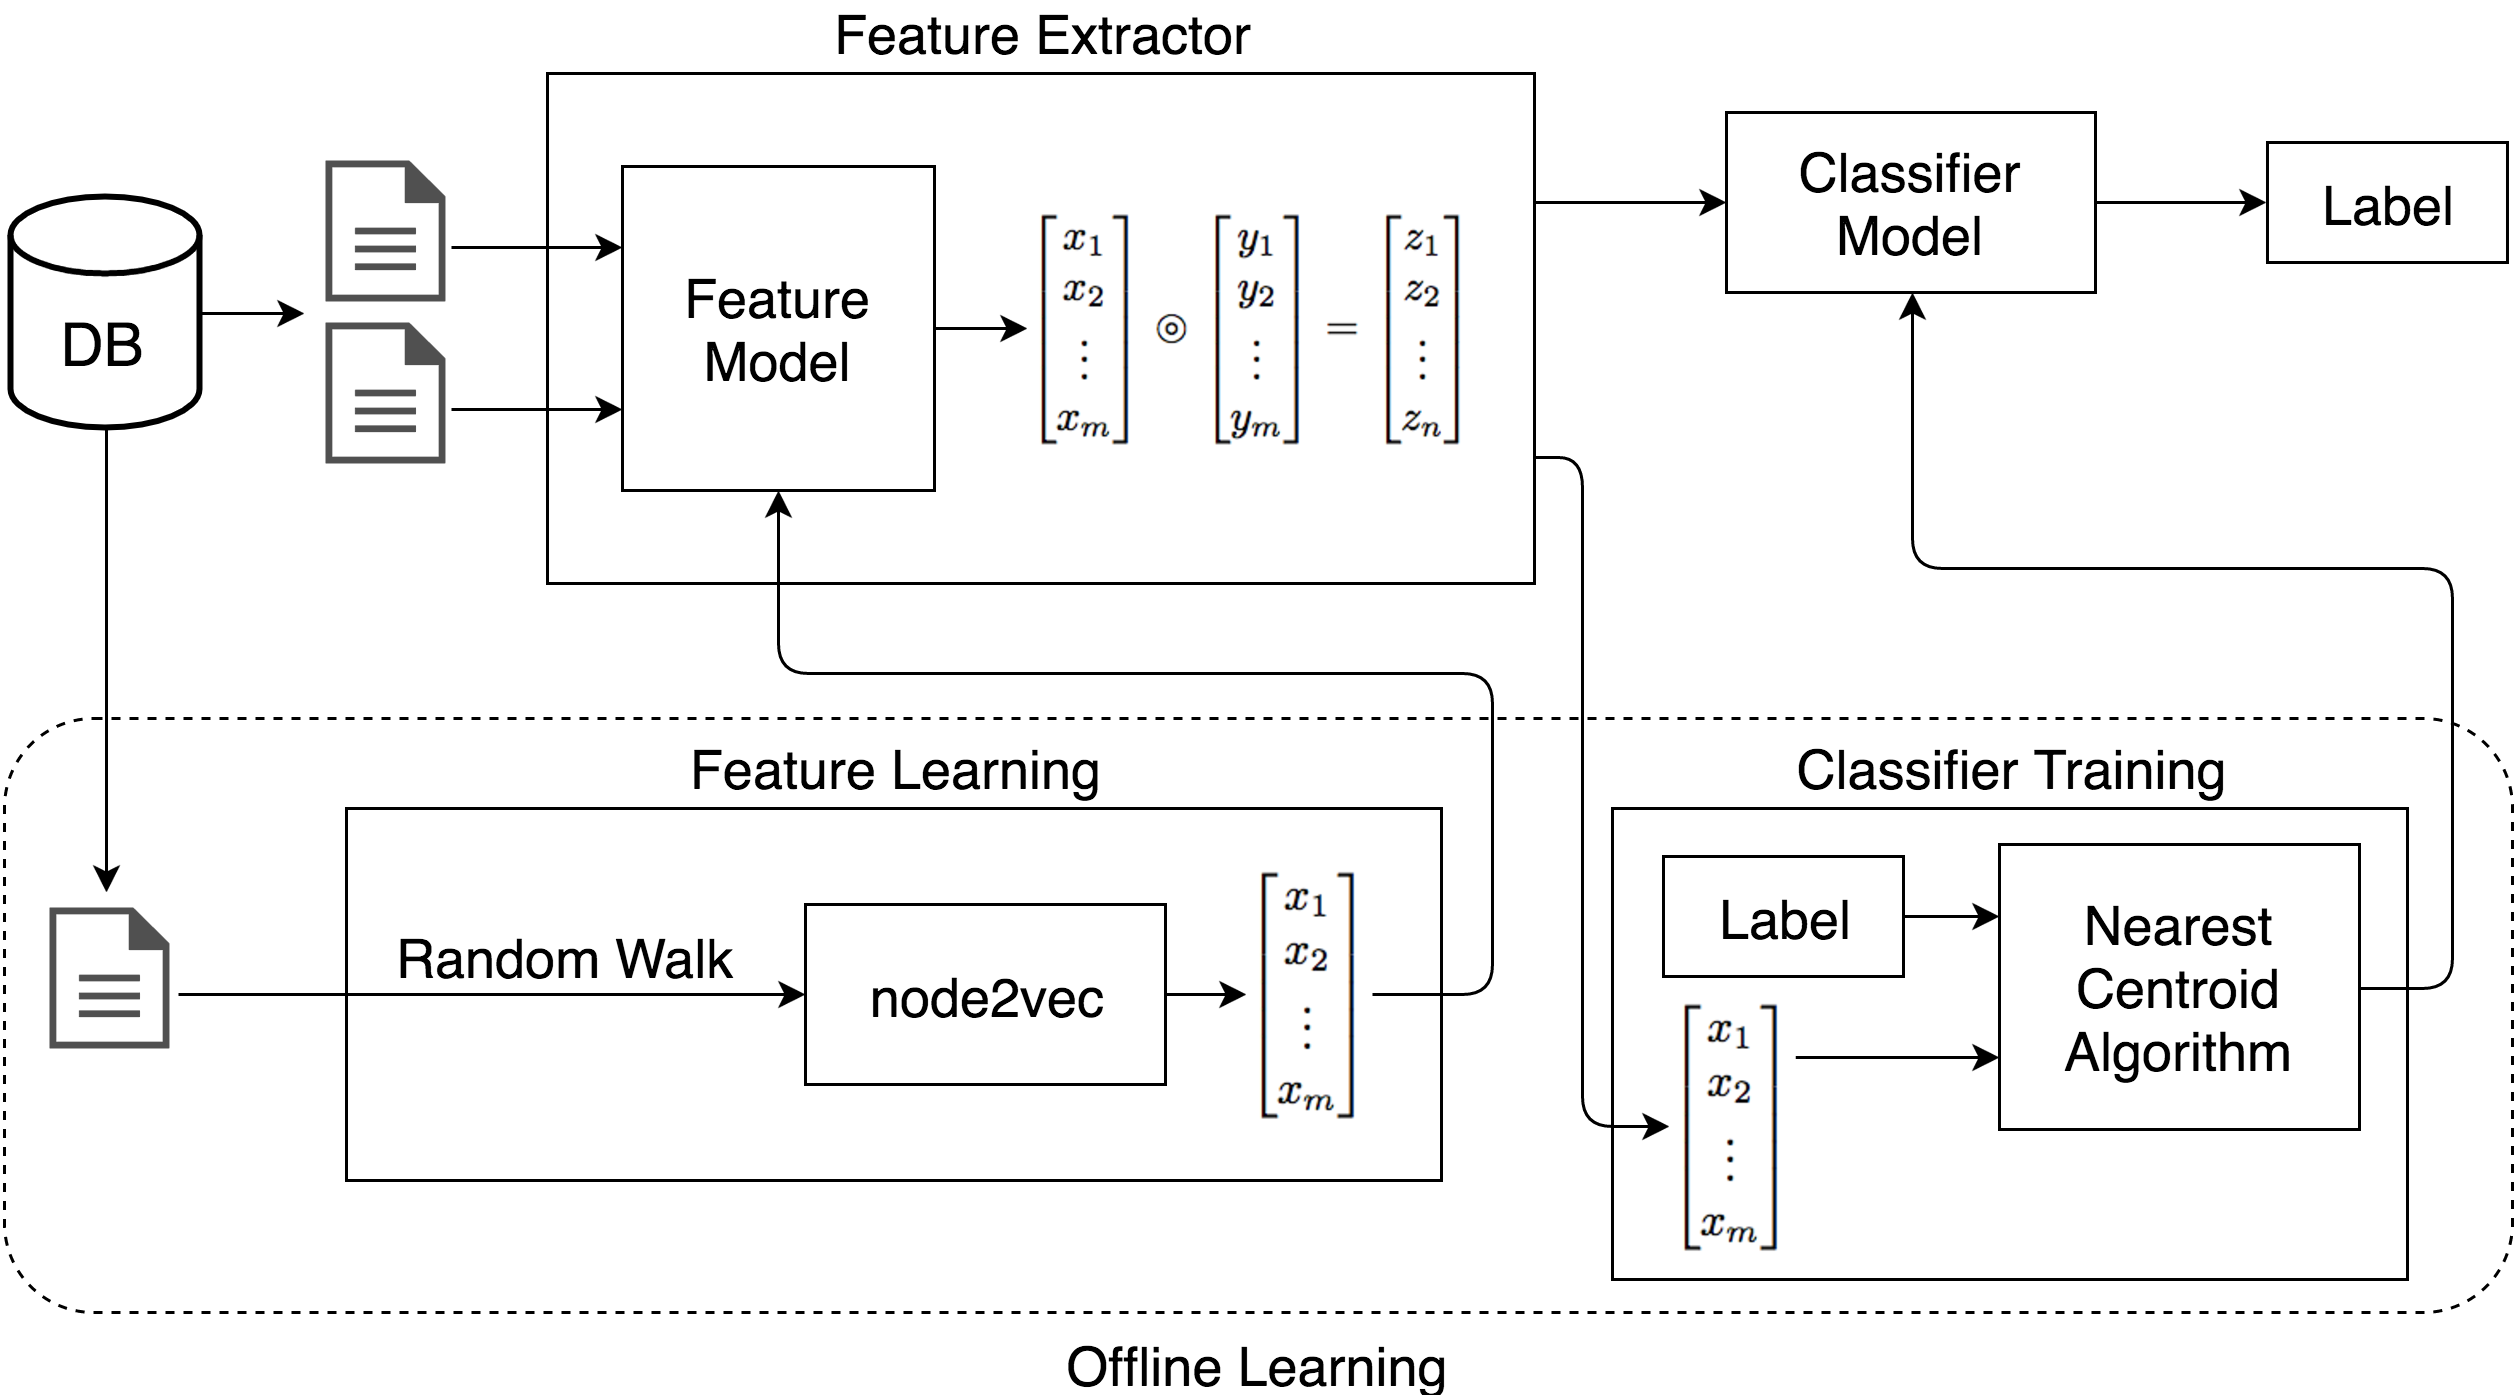
\includegraphics[width=\textwidth]{pipeline2}
\end{frame}
\note{
  \begin{itemize}
    \item Online/Offline Learning
  \end{itemize}
}

\section[UI]{User Interface}
% Første parameter i [] er tekst i header. {} er i indholdsfortegnelsen.

% Slide med emneoverskrift.
\begin{frame}
  \frametitle{}
  \begin{center}
    {\Huge User Interface}
  \end{center}
\end{frame}
\note{
  \begin{itemize}
		\item Notes...
  \end{itemize}
}

% Normal slide:
\begin{frame}
    \frametitle{Some Example Title}
    \framesubtitle{Some example subtitle}
    \centering
    Some text, content, etc.
\end{frame}
\note{
	\begin{itemize}
    \item Notes here...
	\end{itemize}
}
\section[MI Test]{MI Performance}
% Første parameter i [] er tekst i header. {} er i indholdsfortegnelsen.

% Slide med emneoverskrift.
\begin{frame}
  \frametitle{}
  \begin{center}
    {\Huge MI Performance}
  \end{center}
\end{frame}
\note{
  \begin{itemize}
		\item Notes...
  \end{itemize}
}

% Normal slide:
\begin{frame}
    \frametitle{MI Performance}
    %\framesubtitle{Development Method}
    \begin{itemize}
      \item Test Results
      \item Overfitting
      \item Improvements
      \item New Test Results
    \end{itemize}
\end{frame}
\note{
  \begin{itemize}
    \item nerest centroid 97.89
  \end{itemize}
}

% Normal slide:
\begin{frame}
    \frametitle{MI Performance}
    %\framesubtitle{Development Method}
    \begin{figure}[tb]%
    \centering
    \tikzsetnextfilename{barchart}
    \begin{tikzpicture}
      \begin{axis}[
        table/col sep=semicolon,
        xbar=0pt, xmin=0, xmax=1,
        yticklabels from table={10f-results.csv}{name},
        %yticklabel style={text height=1.5ex},
        ytick=data,
        width=0.6\textwidth,
        y=0.4cm,
        enlarge y limits={abs=0.6},
        bar width=4pt,
        /pgf/number format/fixed,
        axis lines*=left,
        xmajorgrids=true,
        legend entries={Recall, Precision},
        legend style={draw=none},
        reverse legend, area legend,
        legend style={at={(1,1.01)},anchor=south east}
      ]
      \addplot [fill=color1!20!white] table [y expr=-\coordindex, x=recall] {10f-results.csv};
      \addplot [fill=color1!70!white] table [y expr=-\coordindex, x=precision] {10f-results.csv};
      \end{axis}
    \end{tikzpicture}
  \end{figure}
\end{frame}
\note{
  \begin{itemize}
    \item nerest centroid 97.89
  \end{itemize}
}

\begin{frame}
    \frametitle{MI Performance}
    %\framesubtitle{Development Method}
    \begin{itemize}
      \item Overfitting
      \begin{itemize}
        \item Poor performance on manually labeled data set
        \item Causation
        \begin{itemize}
          \item Not enough training pairs
          \item Data set contains many end pages such as auto generated pages
        \end{itemize}
      \end{itemize}
    \end{itemize}
\end{frame}
\note{
  \begin{itemize}
    \item Lasse assumption
  \end{itemize}
}


\begin{frame}
    \frametitle{MI Performance}
    %\framesubtitle{Development Method}
    \begin{itemize}
      \item For positive training examples
      \begin{itemize}
        \item For all featured articles a
        \begin{itemize}
          \item select all b where $a \rightarrow b$
          \item add $(a,b)$ to set of training pairs
        \end{itemize}
      \end{itemize}
      \item For negative training examples
      \begin{itemize}
        \item For all featured articles a
        \begin{itemize}
          \item select a random page b where $a \not \rightarrow b$
          \item add $(a,b)$ to set of training pairs
        \end{itemize}
      \end{itemize}
    \end{itemize}
\end{frame}
\note{
  \begin{itemize}
    \item ??
  \end{itemize}
}

\begin{frame}
    \begin{bchart}[step=10,max=100]
        \bcbar{0.4}
            \medskip
        \bcbar{33.4}
            \bigskip
        \bcbar{66.2}
    \end{bchart}
\end{frame}
\note{
  \begin{itemize}
    \item ??
  \end{itemize}
}

\begin{frame}
    \frametitle{MI Performance}
    %\framesubtitle{Development Method}
    \begin{figure}[tb]%
    \centering
    \tikzsetnextfilename{barchart}
    \begin{tikzpicture}
      \begin{axis}[
        table/col sep=semicolon,
        xbar=0pt, xmin=0, xmax=1,
        yticklabels from table={new10f-results.csv}{name},
        %yticklabel style={text height=1.5ex},
        ytick=data,
        width=0.6\textwidth,
        y=0.4cm,
        enlarge y limits={abs=0.6},
        bar width=4pt,
        /pgf/number format/fixed,
        axis lines*=left,
        xmajorgrids=true,
        legend entries={Recall, Precision},
        legend style={draw=none},
        reverse legend, area legend,
        legend style={at={(1,1.01)},anchor=south east}
      ]
      \addplot [fill=color1!20!white] table [y expr=-\coordindex, x=recall] {new10f-results.csv};
      \addplot [fill=color1!70!white] table [y expr=-\coordindex, x=precision] {new10f-results.csv};
      \end{axis}
    \end{tikzpicture}
  \end{figure}
\end{frame}
\note{
  \begin{itemize}
    \item nerest centroid 97.89
  \end{itemize}
}

\section[Dev. Method]{Development Method}
% Første parameter i [] er tekst i header. {} er i indholdsfortegnelsen.

% Slide med emneoverskrift.
\begin{frame}
  \frametitle{}
  \begin{center}
    {\Huge Development Method}
  \end{center}
\end{frame}
\note{
  \begin{itemize}
		\item Notes...
  \end{itemize}
}

% Normal slide:
\begin{frame}
    \frametitle{Development Method}
    %\framesubtitle{Development Method}
    \begin{itemize}
			\item Choice of Paradigm
		  \begin{itemize}
				\item Traditional, analysis-heavy
				\item Agile
			\end{itemize}
			\item Our method
			\begin{itemize}
				\item Self-organized
				\item Responding to change > following a plan
				\item Paper cards and daily status meeting
			\end{itemize}
		\end{itemize}
\end{frame}
\note{
	\begin{itemize}
		\item Analysis-heavy
		\begin{itemize}
			\item Large uncertainties \textrightarrow{} change likely \textrightarrow{} continuous refinement needed
		\end{itemize}
    \item Agile
		\begin{itemize}
			\item Individuals and interactions > processes and tools
			\item Working software > comprehensive documentation
			\item Customer collaboration
			\item Overhead in planning
		\end{itemize}
		\item Any dev. method is infeasible if there is not a consensus for it.
		\item We ended up choosing
		\begin{itemize}
			\item Self-organized method, time allocated for work
			\item We value responding to change > following plan
			\item Task management on paper cards
			\item Daily meetings
		\end{itemize}
	\end{itemize}
}

\section[Reflection]{Reflection}

% Slide med emneoverskrift.
%\begin{frame}
  %\frametitle{}
  %\begin{center}
    %{\Huge Reflection}
  %\end{center}
%\end{frame}
%\note{
  %\begin{itemize}
		%\item Notes...
  %\end{itemize}
%}

% Normal slide:
\begin{frame}
    \frametitle{Reflection}
    \framesubtitle{Development Method}
    \begin{itemize}
			\item Handling data\ \ >\ \ code
			\item Completed a large body of work
		\end{itemize}
\end{frame}
\note{
	\begin{itemize}
    \item Adequate method
			\begin{itemize}
				\item Large part was setting up tools, handling data
				\item less emphasis on ``lots of code''
			\end{itemize}
			\item We completed a large body of work
			\begin{itemize}
				\item handling large dataset, feature engineering, -- learning, classification
				\item Required individual discipline
			\end{itemize}
			\item Towards the end, consistency of artifacts and rituals
			\begin{itemize}
				\item Which showed that we had enough going on and on our minds to dedicate time to method
			\end{itemize}
	\end{itemize}
}

\begin{frame}
    \frametitle{Reflection}
    \begin{itemize}
			\item Difficulty choosing and defining problem
			\item No prior project experience in MI area
			\item Feature Engineering \textrightarrow{} Feature Learning
		\end{itemize}
\end{frame}
\note{
	\begin{itemize}
    \item Notes here...
	\end{itemize}
}

\begin{frame}
    \frametitle{What Have We Learned?}
    \begin{itemize}
			\item Take on manageable projects
			\item Feature engineering is hard
			\item Feature learning is not ``plug and play''
			\begin{itemize}
				\item Not entirely automated
			\end{itemize}
			\item Important to verify subresults in pipeline
			\begin{itemize}
				\item Careful about details and refinement of testing
			\end{itemize}
			\item Long turn-around time (timeboxed project period)
		\end{itemize}
\end{frame}
\note{
	\begin{itemize}
    \item Notes here...
	\end{itemize}
}

\begin{frame}
    \frametitle{Conclusion?}
    \begin{itemize}
			\item ...
		\end{itemize}
\end{frame}
\note{
	\begin{itemize}
    \item Notes here...
	\end{itemize}
}

\section*{}

\begin{frame}
  \frametitle{Overview}
  \tableofcontents
\end{frame}

\end{document}
